\subsection{Evaluation Guide}\label{evaluation-guide}

We sketch how to evaluate the performance of the pipeline on your
reports.

\subsubsection{Create Goldstandard Set}\label{create-goldstandard-set}

One approach is to annotate relevant reports using the existing pipeline
(using the \texttt{annotate} command) and let experts check/complement
the resulting annotations. Alternatively, you can simply convert the
reports to the GATE internal format using the \texttt{import} command.
In this case, the annotator would have to create all annotations
manually, which can be very tedious.

\paragraph{Annotation Guide}\label{annotation-guide}

First, install \href{https://gate.ac.uk/download/}{GATE Developer}.

If you haven't already, load the \texttt{Schema\ Annotation\ Editor} via
\texttt{File} -\textgreater{} \texttt{Manage\ CREOLE\ Plugins}. Tick
\texttt{Load\ now} and \texttt{Load\ always} next to
\texttt{Schema\ Annotation\ Editor}. Restart GATE

Load a schema into GATE: right click on \texttt{Language\ Resources} in
the explorer view, choose \texttt{New} -\textgreater{}
\texttt{Annotation\ Schema}. Click on the briefcase symbol on look for
the
\href{https://github.com/ratschlab/medical-reports-deidentification/blob/main/deidentifier-pipeline/src/main/resources/schemas/master.xml}{master.xml}
file on your filesytem . Open a GATE document, activate
\texttt{Annotation\ Sets} view and select the phi-annotations-manual
annotation set on the right.

Make sure, schemas are loaded in GATE before you open a corpus to
annotate. Load the corpus via \texttt{File} -\textgreater{}
\texttt{Datastores} -\textgreater{} \texttt{Open\ Datastore}. Load
document and add necessary annotations by marking some tokens and
pressing \texttt{Ctrl+E} When creating a new annotation, make sure
\texttt{phi-annotations} is selected on the right hand side. Regularly
do Right-click on document then \texttt{Save\ to\ its\ datastore} (not
done automatically!)

Also make sure reports are read-only to not accidentally edit the
document:

\begin{figure}
\centering
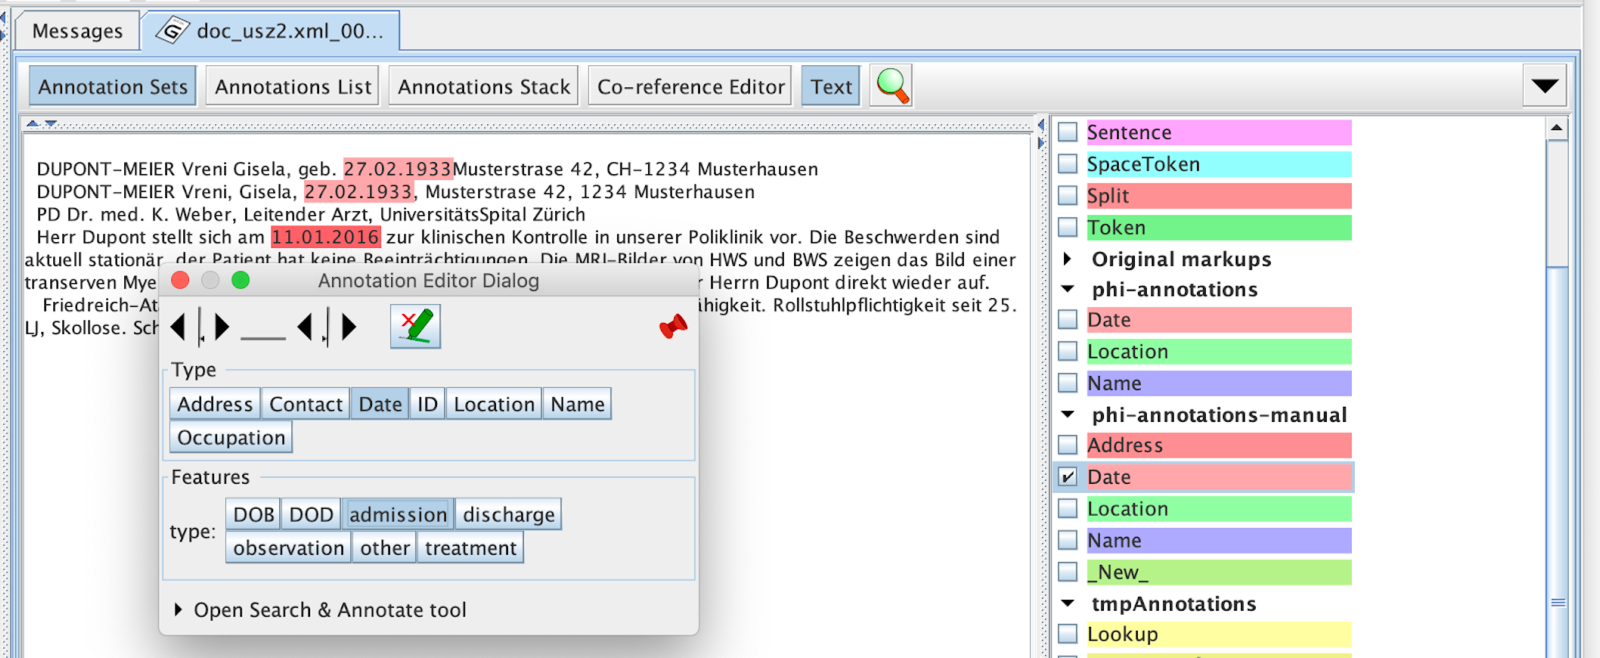
\includegraphics[width=\textwidth]{figs/annotation_dialog.png}
\caption{Annotation View}
\end{figure}

\subsubsection{Evaluate with Respect to Goldstandard
Set}\label{evaluate-with-respect-to-goldstandard-set}

To compare the pipeline output to the goldstandard corpus, annotate the
same reports using the \texttt{annotate} comman, but this time add the
\texttt{-m} option with the path to the goldstandard corpus (\texttt{m}
for ``marked''). You can also add the option
\texttt{-\/-diagnostics-dir} with path where diagnostics information
should be output. It will contain a performance summary in
\texttt{corpus-stats.html} as well detailed output for every report.

\paragraph{Analyse Results in More
Details}\label{analyse-results-in-more-details}

With the \texttt{-\/-diagnostics-dir} option, various ``features'' of
every token are extracted and stored in json files in the
\texttt{ml-features.json}. These features include the annotations of the
pipeline and the rule generating the annotation as well as the
annotations from the goldstandard (if available). They also include in
what lexica a token was found, in what field the token appeared, the
position within the sentence.

These json file(s) can be converted to parquet using a
\href{https://github.com/ratschlab/medical-reports-deidentification/blob/main/scripts/convert_ml_features_to_parquet.py}{python script} and
then explored in a jupyter notebook. This is very helpful to get an
overview over problems in one or several corpora.
